\section{Native tool calls}
\label{sec:native}

\Cref{sec:toolcalls} traced how tool calls moved from lines of text that the application parsed to
structured fields of the model API, and \cref{sec:dispatcher} followed one call through the
dispatcher. This section follows one call across the model API: what makes it native, how its
result returns, how \msa{} reads the formats of two vendors, why a tool that runs inside the harness
keeps the guarantees of a local call, and which controls the application has. The distinction
matters because the model API now fixes the format of every call, while the guarantees about what
runs still come from the harness and from where the tool runs. The section ends with two limits of
native tool calling, which lead to code actions (\cref{sec:codeact}) and to the Model Context Protocol
(Lecture~5).

\subsection{Prompted calling and native tool calling}
\label{sec:native-prompted}

A tool call is native when its format belongs to the model API: the request carries the tool
definitions as a parameter, and the response returns each call in a structured field. The
alternative, prompted calling (\cref{sec:toolcalls}), leaves the format to the application that
calls the model, which in \msa{} is the harness. The prompt describes the tools and an action format
in prose, the model writes each call as a line of text, and the application parses that line.

The weak point of prompted calling is the parser (\cref{lst:native-prompted}). A typical parser
uses a regular expression, a pattern that matches text, to find the tool name and the text between
the brackets. It then splits that text wherever a comma is followed by a space. The listing writes
the edit of \cref{sec:toolcalls} with the three arguments of \demoref{edit}, and the split yields
the path, the old text and the new text, as intended.

If the old text were \demoref{max(i, n)}, the split would cut it in two, and the parser would no
longer find the three arguments in their expected places. Any argument that contains such a comma
breaks the parser in this way. This is the failure of prompted calling that \cref{sec:toolcalls}
described.

\begin{lstlisting}[basicstyle=\ttfamily\footnotesize, caption={Illustrative code for prompted calling. The application finds the call in the model's text and splits the arguments at each comma followed by a space.}, label=lst:native-prompted]
# the model writes a line of text:
#   Action: edit[src/parse.py, i <= n, i < n]
m = re.match(r"Action: (\w+)\[(.*)\]", line)
name, args = m[1], m[2].split(", ")
\end{lstlisting}

In \cref{lst:native-native}, the request passes the tool definitions in the parameter
\demoref{tools}, and the reply returns the calls in the field \demoref{tool\_calls} of OpenAI's Chat
Completions API. The name and the arguments of each call sit in separate fields, so the application
no longer searches the model's text for them \citep{openai-function-calling}. Prompted calling was
the common pattern in 2022. OpenAI introduced native tool calling in June 2023, with models fine-tuned to
detect when a function needs to be called and to reply with JSON that follows the function's
signature \citep{openai2023functioncalling}. Anthropic followed with an equivalent format.

\begin{lstlisting}[basicstyle=\ttfamily\footnotesize, caption={Illustrative code for native tool calling, abbreviated from OpenAI's Python client. The request carries the tool definitions, and the reply holds each call in a structured field.}, label=lst:native-native]
# the request carries the tool definitions
r = client.chat.completions.create(
        model=..., messages=msgs, tools=[...])
# the reply holds the calls in a structured field
call = r.choices[0].message.tool_calls[0]
name = call.function.name
args = json.loads(call.function.arguments)
\end{lstlisting}

Native tool calling moves the parsing of calls from the application to the provider, which owns both the
format and its parser. Every application therefore receives the same structured result. The
provider turns the tool definitions into a prompt for the model, and it parses the model's output
into the structured fields of the reply. Anthropic's API, for example, builds a special system
prompt from the tool definitions, and that prompt tells the model that its output is parsed with
regular expressions \citep{anthropic-define-tools}.

The application still decodes the arguments of each OpenAI call. OpenAI sends them as a JSON string,
which the last line of \cref{lst:native-native} decodes. Without strict mode (\cref{sec:toolcalls}),
that string can be malformed, and decoding it then fails. With strict mode, a complete argument
string always decodes and matches the tool's argument schema (\cref{sec:native-arguments}).

\subsection{Returning each result by its call identifier}
\label{sec:native-ids}

\begin{figure}[t]
  \centering
  \begin{tikzpicture}[
    life/.style={densely dotted, draw=ibmfg!45},
    elab/.style={lab, font=\sffamily\footnotesize, inner sep=1.5pt},
    evnum/.style={circle, fill=ibmfg!85, text=white, inner sep=1pt, minimum size=3.8mm,
      font=\sffamily\scriptsize\bfseries},
    act/.style={draw=ibmfg!60, rounded corners=2pt, fill=black!4, font=\sffamily\footnotesize,
      inner sep=2pt}
  ]
    \node[mnode, minimum width=15mm] (h) at (0,0) {harness};
    \node[mnode, minimum width=15mm] (m) at (3.9,0) {model API};
    \node[rnode, minimum width=15mm] (t) at (7.0,0) {tool};
    \foreach \n in {h,m,t} { \draw[life] (\n.south) -- ++(0,-5.65); }

    % first request and the reply that ends in a call
    \draw[flow] (0,-1.0) -- node[elab, above] {messages + tool definitions} (3.9,-1.0);
    \node[evnum] at (-0.75,-1.0) {1};
    \draw[back] (3.9,-2.0) -- node[elab, above, align=center]
      {tool call, id \texttt{call\_7}\\finish reason: \texttt{tool\_calls}} (0,-2.0);
    \node[evnum] at (-0.75,-2.0) {2};

    % the dispatch cycle runs in the harness
    \node[act] at (0.75,-2.6) {find, bind, check};
    \draw[flow] (0,-3.3) -- node[elab, above, pos=0.72] {run \texttt{edit}} (7.0,-3.3);
    \draw[back] (7.0,-3.9) -- node[elab, above, pos=0.72] {result} (0,-3.9);
    \node[evnum] at (-0.75,-3.3) {3};

    % second request: the result repeats the identifier
    \draw[flow] (0,-4.85) -- node[elab, above, align=center]
      {messages + result\\\texttt{tool\_call\_id}: \texttt{call\_7}} (3.9,-4.85);
    \node[evnum] at (-0.75,-4.85) {4};
    \draw[back] (3.9,-5.55) -- node[elab, above] {final answer} (0,-5.55);
    \node[evnum] at (-0.75,-5.55) {5};
  \end{tikzpicture}
  \caption{One native tool call as two requests to the model API. The first reply ends in a call
  with the identifier \texttt{call\_7}. The harness runs the call and returns its result in a
  second request that repeats the identifier.}
  \label{fig:native-roundtrip}
\end{figure}

\begin{table*}[t]
  \caption{The native tool-call formats of OpenAI's Chat Completions API and Anthropic's Messages
  API, one row per part of the round trip of \cref{fig:native-roundtrip}. Both formats have every
  part except the error flag, which only Anthropic's result block carries.}
  \label{tab:native-formats}
  \begin{adjustbox}{width=\linewidth}\begin{tabularx}{\linewidth}{L{0.17\linewidth}XX}
    \toprule
    \textbf{Part} & \textbf{OpenAI Chat Completions} & \textbf{Anthropic Messages} \\
    \midrule
    \textbf{Tool definition, in the request} & An entry in \demoref{tools} with
    \demoref{"type":\ "function"} and a \demoref{function} object holding \demoref{name},
    \demoref{description}, \demoref{parameters} and, optionally, \demoref{strict} & An entry in
    \demoref{tools} holding \demoref{name}, \demoref{description}, \demoref{input\_schema} and,
    optionally, \demoref{strict} \\ \addlinespace[3pt]
    \textbf{Call, in the response} & An entry in \demoref{tool\_calls} holding
    \demoref{function.name} and \demoref{function.arguments}, a JSON string & A
    \demoref{tool\_use} block holding \demoref{name} and \demoref{input}, a JSON object \\ \addlinespace[3pt]
    \textbf{Call identifier} & \demoref{id} of the entry, such as \demoref{call\_7} &
    \demoref{id} of the block, such as \demoref{toolu\_01} \\ \addlinespace[3pt]
    \textbf{Signal that the reply ends in calls} & \demoref{finish\_reason} is
    \demoref{tool\_calls} & \demoref{stop\_reason} is \demoref{tool\_use} \\ \addlinespace[3pt]
    \textbf{Result, in the next request} & A message with \demoref{"role":\ "tool"}, the
    \demoref{tool\_call\_id} and the \demoref{content} & A \demoref{tool\_result} block with the
    \demoref{tool\_use\_id} and the \demoref{content}, placed first in a user message \\ \addlinespace[3pt]
    \textbf{Error flag on the result} & No separate field & Optional \demoref{is\_error} \\
    \bottomrule
  \end{tabularx}\end{adjustbox}
\end{table*}

Each native call carries a \textbf{call identifier}, an id that the call's result must repeat. The
harness returns the result in a message that carries the same id, so the identifier pairs each
result with its call. The pairing matters when one reply holds several calls, which parallel tool
calls allow (\cref{sec:toolcalls}).

\Cref{fig:native-roundtrip} shows one native call as two requests to the model API. Its numbered
steps are the following:
\be
\item \textbf{First request.} The harness sends the conversation so far, its messages, together with
the tool definitions.
\item \textbf{Call.} The model API replies with a tool call that carries the identifier
\demoref{call\_7}. The reply's finish reason, a field that says why the model stopped writing, is
\demoref{tool\_calls}. It tells the harness that the reply ends in a request for tools and holds no
final answer.
\item \textbf{Dispatch.} The harness runs the dispatch cycle of \cref{sec:dispatcher}: it finds the
tool, binds the arguments, checks the request, runs \demoref{edit} and observes the result. The
figure groups the checks before the run. In \msa{}, the dispatcher's own checks, a registered name
and arguments that bind, come first, and the path check runs as the first step inside
\demoref{edit}, before any write.
\item \textbf{Second request.} The harness sends the messages again, now with the result, keyed by
the identifier \demoref{call\_7}.
\item \textbf{Answer.} The model API replies with a final answer.
\ee

Every call needs a result. Anthropic's API rejects a request in which a tool call of the previous
reply is not followed immediately by its result \citep{anthropic-handle-tool-calls}. The harness of
\msa{} meets this rule by returning a tool message (\cref{sec:dispatcher}) for every call that the
tools node receives, including a call that the dispatcher refused. A refusal is itself an
observation, so it can serve as the call's result, and the model reads the reason for the refusal.

A call receives no result in the following cases:
\bi
\item \textbf{Arguments that cannot be decoded.} LangChain's chat-model adapter, which \msa{}
uses to call the model (\cref{sec:native-adapters}), puts a call whose argument string is malformed
into a separate list of invalid tool calls. The tools node does not read that list, so no tool
message answers the call.
\item \textbf{An exception that escapes the dispatcher.} An exception that the dispatcher does not
catch ends the run (\cref{sec:dispatcher}), so no result is ever sent.
\ei

Everything that happens between the two requests is harness code. The model proposes calls. The
harness decides whether each call runs, runs it, and decides which result the model receives. The
model never executes a tool, and it never writes a result.

\subsection{The OpenAI and Anthropic formats}
\label{sec:native-vendors}

\begin{figure*}[t]
  \centering
  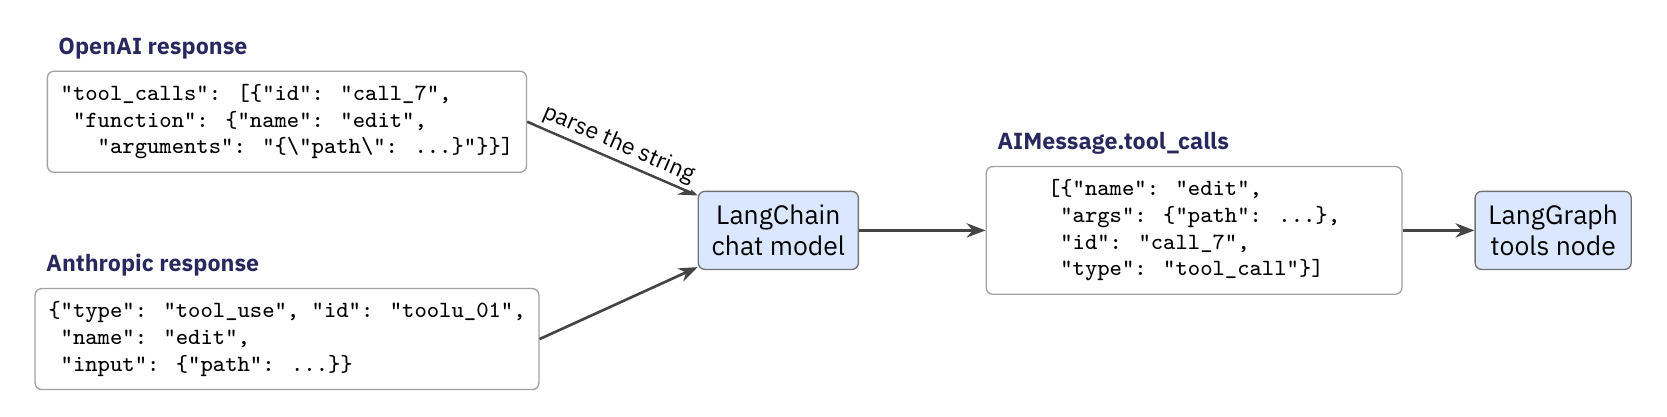
\includegraphics[width=0.92\textwidth]{figures/deck/3e51a79c67.png}
  \caption{LangChain's chat-model adapter converts an OpenAI reply and an Anthropic reply into
  one list, \texttt{AIMessage.tool\_calls}, which the tools node of the harness reads. The OpenAI
  arguments arrive as a string and are decoded on the way, and the Anthropic input arrives as an
  object and is copied.}
  \label{fig:native-adapters}
\end{figure*}

The native formats of OpenAI and Anthropic differ in their field names and agree in their
structure. Each has a tool definition in the request, a call with an identifier in the response,
and a result in the next request that repeats the identifier
\citep{openai-function-calling,anthropic-tooluse}. \Cref{tab:native-formats} sets the two formats
side by side. Each row names one part of the round trip, and its two cells give that part in each
vendor's format. The last row holds the one part that only Anthropic's format has.

The differences that matter to a harness are the following:
\bi
\item \textbf{Arguments.} OpenAI sends the arguments as a JSON string, which must be decoded before
the arguments can be bound. In \msa{}, LangChain's adapter decodes it (\cref{sec:native-adapters}).
Anthropic sends the arguments as a JSON object, which needs no decoding.
\item \textbf{Placement of results.} In OpenAI's format, the harness returns each result as a
message of its own, with the role \demoref{tool}. In Anthropic's format, the harness places the
results as \demoref{tool\_result} blocks inside a user message, and these blocks must come before
any text in that message.
\item \textbf{Errors.} Anthropic's result block has an optional flag, \demoref{is\_error}, that marks
a failed call. OpenAI's result message has no such field.
\ei

OpenAI's newer Responses API has the same parts under other names. A call is a
\demoref{function\_call} item with a \demoref{call\_id}, and its result is a
\demoref{function\_call\_output} item that repeats the \demoref{call\_id}.

\subsection{One list of calls for both formats}
\label{sec:native-adapters}

The harness of \msa{} never reads a vendor's format directly. It is built on LangGraph, a library
that runs an agent as a graph of nodes, and it calls the model through LangChain's chat-model
adapters, the classes through which LangChain calls each vendor's API. These adapters convert each
vendor's reply into one common message object, an
\demoref{AIMessage} \citep{langchain-messages}. Its attribute \demoref{tool\_calls} is a list with
one entry per call, and each entry holds the call's name, its arguments as a dictionary
(\demoref{args}) and its identifier (\demoref{id}).

\Cref{fig:native-adapters} follows both replies into the one list. For OpenAI, the adapter
decodes the argument string into the dictionary. For Anthropic, it copies the input object, which is
already a dictionary. A call whose arguments cannot be decoded goes to a separate list,
\demoref{invalid\_tool\_calls}. This is the case of \cref{sec:native-ids} in which a call receives
no result.

LangGraph runs the graph, and its tools node reads only the list \demoref{tool\_calls}. The same
harness code therefore runs with either vendor, and none of the code written for the harness handles
a vendor's format.

The tools node turns the list into results with a short loop (\cref{lst:native-toolsnode}). The
first line reads the list from the last message in the state record, which stores the run's
variables (Lecture~3). That last message is the model's reply. For each call, the loop passes the
name and the arguments to the dispatcher, which returns an observation. It then builds one tool
message per call, which LangChain calls a \demoref{ToolMessage}. The message's content is the
observation's result, and its \demoref{tool\_call\_id} repeats the call's identifier.

\begin{lstlisting}[basicstyle=\ttfamily\footnotesize, caption={Illustrative code for the loop of the tools node, abbreviated. Each call goes to the dispatcher, and each observation returns to the model as one tool message keyed by the call's identifier.}, label=lst:native-toolsnode]
for call in state["messages"][-1].tool_calls:
    observation = dispatcher(
        {"name": call["name"], "args": call["args"]})
    replies.append(ToolMessage(
        content=observation.result,
        tool_call_id=call["id"],
        name=call["name"]))
\end{lstlisting}

The loop runs the calls one after another, in the order in which they appear in the reply. Each
call finishes before the next one begins, so the effects of the calls follow their order in the
reply. If one reply asks for two edits of the same file, the second edit sees the file as the first
one left it.

\subsection{Guarantees of in-process tools}
\label{sec:native-local}

A tool that runs inside the harness's own process gives each call the guarantees of a local call,
as long as the harness runs one call at a time. We call such a tool an \textbf{in-process tool}. The
tools of \msa{}, \demoref{read\_file}, \demoref{search} and \demoref{edit}, are in-process tools. A
local call, as defined in \cref{sec:toolcalls}, is a call to a procedure in the caller's own
process.

Such a call has the following properties. The grouping is the course's own, and no single source
lists the properties together.
\bi
\item \textbf{A returned call shows that the tool ran.} When the tool function returns, the
dispatcher holds its result. When the function fails, the dispatcher holds the exception it raised.
Every call that reaches the tool function ends in one of these two outcomes, unless the tool hangs,
and the harness knows which one.
\item \textbf{One call runs the tool once.} No retry and no duplicate delivery sit between the
dispatcher and the tool. The retried request of \cref{sec:toolcalls}, which applied the same patch
twice, cannot occur inside one process.
\item \textbf{The harness and the tool fail together.} The tool is a function in the harness's
process. If the process crashes, both stop, so neither can keep running after the other has failed.
\item \textbf{No timeout is needed.} A tool that hangs also hangs the harness. The harness therefore
never has to guess whether a slow call has failed.
\item \textbf{Partial effects are visible.} A \textbf{partial effect} is a change that an operation
made before it failed. The tool and the harness share the files of the workspace, so the harness can
inspect what a failed tool changed and repair it.
\item \textbf{Effects happen in program order.} \textbf{Program order} means that effects occur in
the order of the calls in the reply. The tools node runs the calls of a reply one after another
(\cref{sec:native-adapters}).
\ei

No timeout is needed because a local caller never has to tell a slow callee from a dead one. Across
a boundary, a reply that has not arrived may mean that the callee is slow, that it has crashed, or
that the reply was lost (\cref{sec:toolcalls}). The caller must then choose how long to wait before
it gives up. A local call can still hang. A tool function that never returns blocks the whole
harness, and \cref{sec:codeact} returns to this problem, because one code action can hold any amount
of computation.

These guarantees come from where the tool runs and from how the harness runs it. The native format
contributes none of them, so prompted calling with an in-process tool has the same properties. They
hold only under the following conditions:
\bi
\item \textbf{The tool runs inside the harness.} A tool in another process, such as a tool that an
MCP server offers (\cref{sec:toolcalls}), receives each call as a message, and a message can be lost,
delayed or delivered twice.
\item \textbf{The harness runs one call at a time.} Parallel tool calls let a model place several
calls in one reply. A harness that ran them concurrently would lose program order.
\ei

Each of these properties can fail when a call crosses to another machine, because a remote call
differs from a local one in the ways that \cref{sec:toolcalls-rpc} listed, partial failure among
them \citep{waldo1994note}. Remote procedure calls kept the semantics of a local call where they could and
gave communication failures semantics of their own \citep{birrell1984rpc}. Results from distributed
computing explain why several of these properties are lost across a boundary:
\bi
\item \textbf{Ordering (program order).} Within one process, events are ordered by the sequence in which the process
executes them. Events in different processes can be ordered only through the messages between them
\citep{lamport1978time}. Inside the harness, the sequence of the calls alone therefore fixes their
order.
\item \textbf{Agreement (a returned call shows that the tool ran).} Two parties that communicate over a channel that can lose messages can
never both be certain of an outcome, a result known as the Two Generals problem
\citep{akkoyunlu1975constraints,gray1978notes}. A local call involves no such channel.
\item \textbf{Failure classes (failing together, no timeout needed).} A server can fail by omitting a reply, by replying too early or too
late, by replying with a wrong value, by crashing, or in arbitrary ways
\citep{cristian1991understanding}. A remote caller must allow for each of these failures.
\item \textbf{Repair (partial effects are visible).} An effect that has already been made permanent cannot simply be cancelled. A
later step, called compensation, must undo it \citep{garciamolina1987sagas}. An in-process tool lets
the harness inspect and repair the files directly.
\ei

\subsection{Requiring or forbidding tool calls}
\label{sec:native-choice}

\begin{table}[t]
  \caption{Request parameters with which an application controls tool calls in OpenAI's Chat
  Completions API and Anthropic's Messages API.}
  \label{tab:native-controls}
  \begin{adjustbox}{width=\linewidth}\begin{tabularx}{\linewidth}{L{0.24\linewidth}XX}
    \toprule
    \textbf{Control} & \textbf{OpenAI} & \textbf{Anthropic} \\
    \midrule
    \textbf{Require a call} & \demoref{tool\_choice} set to \demoref{"required"} or to a named
    function & \demoref{tool\_choice} of type \demoref{any} or \demoref{tool}, rejected by several
    of the newest Claude models and by any model on which extended thinking is turned on manually \\ \addlinespace[3pt]
    \textbf{Forbid calls} & \demoref{tool\_choice} set to \demoref{"none"} &
    \demoref{tool\_choice} of type \demoref{none} \\ \addlinespace[3pt]
    \textbf{At most one call per reply} & \demoref{parallel\_tool\_\allowbreak calls} set to false
    & \demoref{disable\_parallel\_\allowbreak tool\_use} set to true \\ \addlinespace[3pt]
    \textbf{Schema-valid arguments} & \demoref{"strict":\ true} in the tool definition &
    \demoref{"strict":\ true} in the tool definition \\
    \bottomrule
  \end{tabularx}\end{adjustbox}
\end{table}

The application can tell the model API whether a reply must contain a tool call, may contain one,
or must contain none. The request parameter that does this is called \textbf{tool choice}: it
requires, allows or forbids tool calls. Requiring a call is called \textbf{forced tool use}, and it
demands a call to some tool or to a named tool. \Cref{tab:native-controls} lists the parameters of
both vendors, together with the controls of \cref{sec:native-arguments}.

Both vendors accept the setting \demoref{auto}, which lets the model decide, and the setting
\demoref{none}, which forbids calls. OpenAI's Chat Completions API requires a call with
\demoref{required}, or with a named function when one particular tool must be called
\citep{openai-function-calling}. Anthropic's API requires a call with \demoref{any}, which demands
some tool, or with \demoref{tool}, which demands a named tool \citep{anthropic-define-tools}.

Requiring a call suits a task that must always produce structured output, such as extracting the
fields of an invoice. The application defines a tool whose arguments are those fields, for example
one named \demoref{record\_invoice}. With OpenAI, it forces a call to that tool. Every reply then
contains the call, and the call's arguments are the extracted fields in the shape that the argument
schema fixes.

Anthropic restricts forcing. Several of the newest Claude models reject forced tool use whatever
their settings. So does any Claude model on which the application has turned on extended thinking
manually, a setting in which the model reasons at length before it replies.

On these models, the alternative is \demoref{auto} together with strict mode, which Anthropic calls
strict tool use, or structured outputs, a feature that makes the whole reply follow a fixed JSON
schema. With \demoref{auto}, the model may still answer without calling the tool. Strict mode then
guarantees only that the arguments are valid whenever the model does call it.

Forbidding calls works with both vendors and with every Claude model, and it suits the end of a
budgeted run. In Lecture~3's budgeted loop, a run may make only a fixed number of model calls, 40 in
\msa{}. The harness can make the last call that the budget allows with tool choice set to
\demoref{none}. The model then cannot request another tool, so the run ends with a text answer.
Without this setting, the model could request a tool on that last call, and the tool's result would
never reach the model.

\subsection{Limiting calls and their arguments}
\label{sec:native-arguments}

% A figure* floats to the top of a later page, so it is placed here to appear beside
% \cref{sec:native-limits}, which uses it.
\begin{figure*}[t]
  \centering
  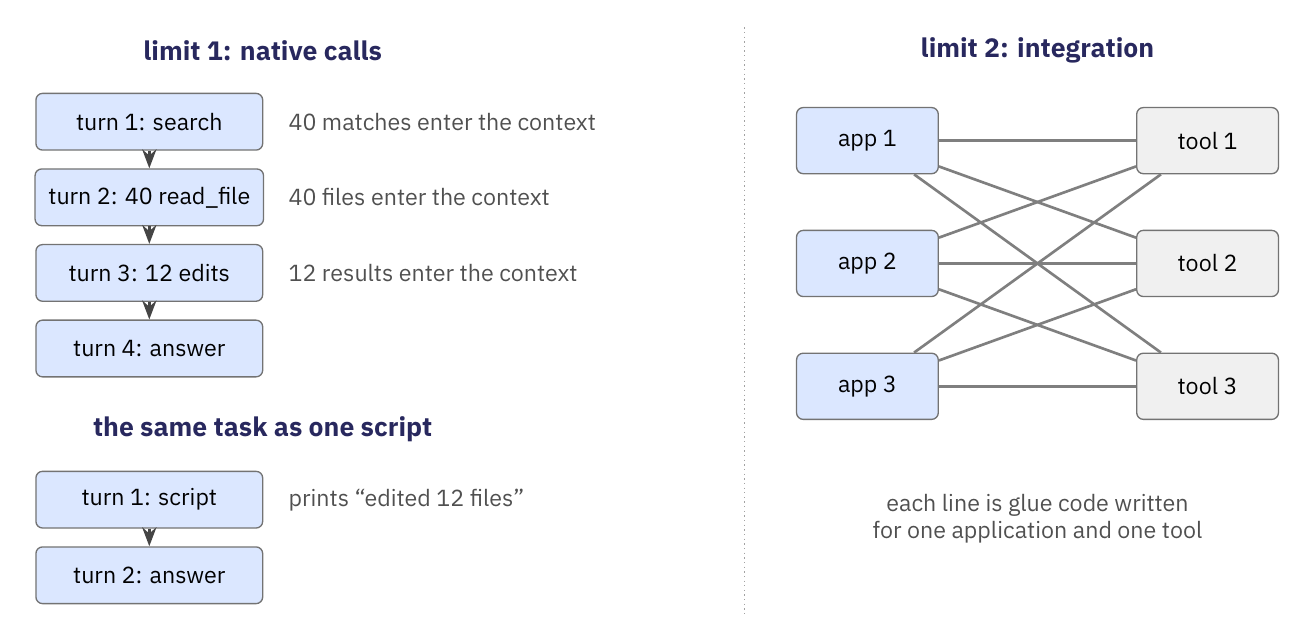
\includegraphics[width=0.78\textwidth]{figures/deck/6eec671dd0.png}
  \caption{Left: a task that edits only the files in which a search match lies inside a loop of the
  source code, done with native calls and done as one script, with illustrative numbers. Right:
  three applications and three tools, where each line is integration code written for one
  application and one tool.}
  \label{fig:native-limits}
\end{figure*}

Further request parameters limit how many calls a reply may hold and which arguments a call may
carry. Disabling parallel tool calls limits each reply to at most one call. OpenAI does this with the
parameter \demoref{parallel\_tool\_calls} set to false. Anthropic does it with the field
\demoref{disable\_parallel\_tool\_use} set to true inside the tool choice \citep{anthropic-tooluse}.

One call per reply serves edits that depend on one another and must run in order. Each edit then
runs, and its result returns, before the model asks for the next one. Program order then no longer
depends on how the harness runs the calls of a reply, because no reply holds more than one call.
The cost is extra turns. A turn is one pass through the loop, from one model call to the next
(Lecture~2), and work that a single reply could have requested now takes one turn per tool call.

Strict mode guarantees that the arguments of a call match the tool's argument schema. Without it, a
call may carry an argument of the wrong type, for example \demoref{\{"path":\ 7, ...\}} where the
schema requires the path to be a string. Both vendors offer strict mode as a flag,
\demoref{"strict":\ true}, on the tool definition, and both implement it by constrained decoding
\citep{openai-function-calling,anthropic-strict-tool-use}.

In \textbf{constrained decoding}, at each step of generation, the model may choose only tokens that
keep the output valid under the schema \citep{openai2024structuredoutputs}. A model normally samples
each token from its whole vocabulary. Under constrained decoding, every token that would break the
schema is excluded, so arguments that the model finishes decode and match the schema. The
guarantee does not cover a reply that is cut off early, for example at the reply's length limit, or
a reply in which the model refuses the request. Anthropic also documents that strict mode does not
guarantee capitalization when the schema restricts a string to a fixed list of values, an enum. A
returned value can then differ from a listed value in its capital letters
\citep{anthropic-structured-outputs}.

The guarantee holds only within the subset of JSON Schema that strict mode supports, and a request
whose schema leaves that subset is rejected. OpenAI's strict mode, for example, requires
\demoref{"additionalProperties":\ false}, which forbids fields that the schema does not list, and it
requires every property to be listed as required. Anthropic's strict mode accepts properties that
are not required.

Each vendor thus accepts a different subset, so the subset becomes part of the tool's contract. The
argument schema must be written within it, and a tool moved to another vendor may need its schema
rewritten.

The guarantee also covers only the shape of the arguments (\cref{sec:toolcalls}). A call whose path
is a string, as the schema demands, can still name the wrong file.

\subsection{Limits of native tool calling}
\label{sec:native-limits}

Native tool calling is limited in what one reply can express and in how a tool reaches the applications
that use it. The first limit is that a reply cannot loop or branch. A reply is a list of calls that
the model fixes when it writes the reply. It cannot say ``for every match, read the file'', and it
cannot say ``if the match lies inside a loop of the code, edit the file''.

Every decision that depends on a result therefore costs a turn. Every result also enters the model
context, what one model call receives (Lecture~3).

\Cref{fig:native-limits} shows both limits. Its left side counts the turns of one task done with
native calls and done as one script, and its right side draws the integration code between three
applications and three tools. The task edits only the files in which a search match lies inside a
\texttt{for} or \texttt{while} loop of the source code.

With native calls, the first turn searches, and all the matches enter the model context. The second turn
reads every matching file, and every file enters the model context. Parallel tool calls let the model
batch these reads into one reply, but the choice of the files to edit still waits for the next turn.
The third turn edits the files that qualify, and the fourth turn answers.

Suppose instead that the model could write a script, a short program that the harness runs
(\cref{sec:codeact}). The script makes the same decisions within one turn and prints only a summary,
such as the number of files it edited. Every result that passes through the model context costs tokens and
time. The script keeps those results out of the model context and needs fewer turns.

The second limit is that each application integrates each tool itself, in its own language and in
its vendor's format. Every pair of an application and a tool needs its own integration code, so
three applications and three tools need nine pieces of it.

Code actions address the first limit: the model writes a program, which can loop and branch over
results within one turn (\cref{sec:codeact}). The Model Context Protocol addresses the second: a
server offers its tools once, through one protocol, and any application that speaks the protocol can
list and call them. Lecture~5 studies the protocol, and the end of \cref{sec:codeact} returns to the
integration problem.

\subsection*{Key points}
\bi
\item A tool call is native when the model API defines its format: the request carries the tool
definitions, the reply returns each call in a structured field, and the provider builds the prompt
from the definitions and parses the model's output.
\item Every native call carries a call identifier that its result must repeat, and the harness of
\msa{}, which alone decides whether a call runs, returns a tool message for every call it receives,
refused calls included.
\item OpenAI's and Anthropic's formats differ in field names and share a tool definition, a call with
an identifier and a result that repeats it, and LangChain converts both into the one list that the
tools node reads.
\item An in-process tool that the harness runs one call at a time gives each call the guarantees of
a local call, whether the call is native or prompted: a returned call shows that the tool ran, one
call runs the tool once, harness and tool fail together, no timeout is needed, partial effects are
visible, and effects follow program order.
\item Tool choice requires, allows or forbids tool calls, and disabling parallel tool calls keeps
program order at the cost of extra turns.
\item Strict mode uses constrained decoding to make the arguments match the argument schema, within
the subset that the vendor supports, and a call that matches the schema can still name the wrong
file.
\item A native reply cannot loop or branch, which code actions address, and each application must
integrate each tool itself, which the Model Context Protocol addresses.
\ei
